\documentclass[border=10pt]{standalone}

\usepackage{tikz}
\usepackage{tikzsymbols}
\usetikzlibrary{calc,patterns,shapes.geometric}

\def\centerarc[#1](#2)(#3:#4:#5){\draw[#1] ($(#2)+({#5*cos(#3)},{#5*sin(#3)})$) arc (#3:#4:#5);}

\begin{document}
	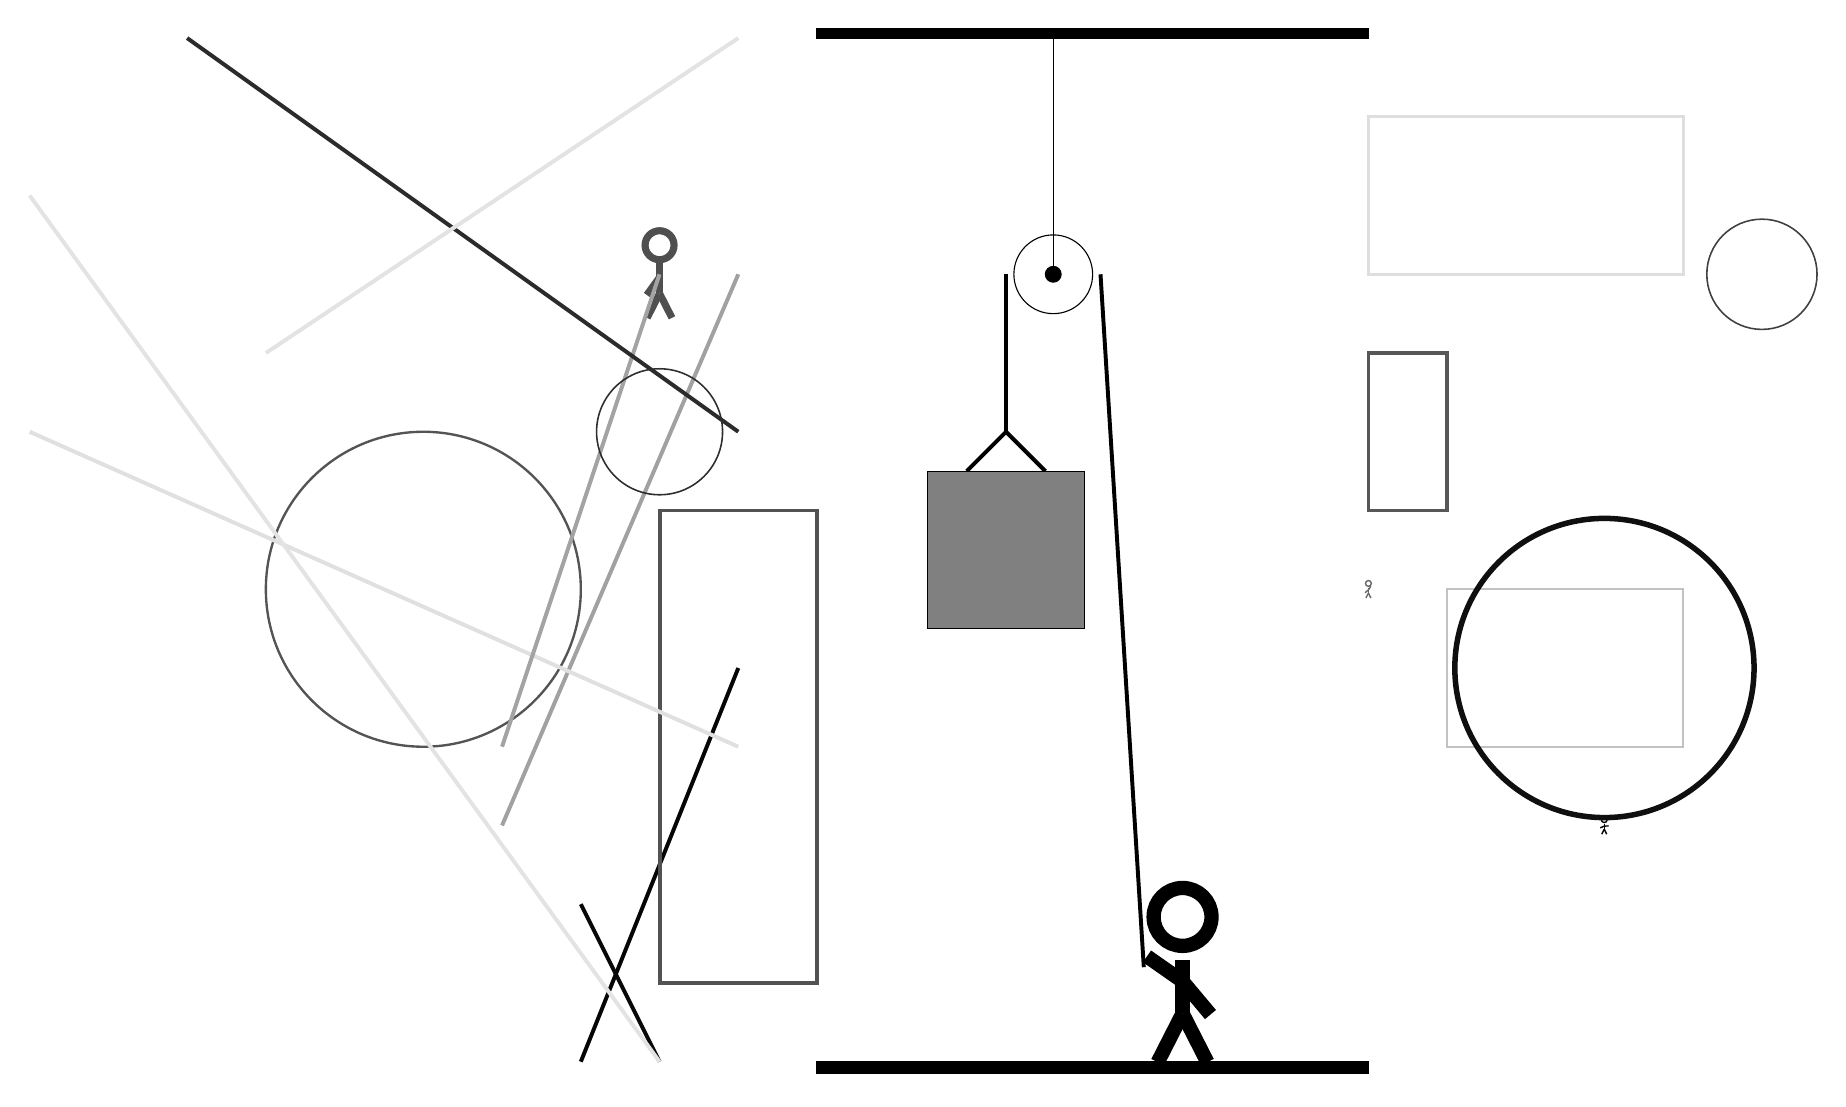
\begin{tikzpicture}
		%%%%% START %%%%%
		
		\draw[fill=black] (-2, 10) rectangle (5, 10.125);
		
		\node[line width=0.3mm, color=black!97] at (8, 0) {\Strichmaxerl[1][24][2]};
		
		\node[line width=0.4mm, color=black!69] at (-4, 7) {\Strichmaxerl[5][54][90]};
		\draw[line width=0.4mm, color=black!66] (6, 6) rectangle (5, 4);
		\draw [line width=0.2mm, color=black!75](10, 7) circle (0.7);
		\draw[line width=0.5mm, color=black!98](-3, 2) -- (-5, -3);
		\draw[line width=0.5mm, color=black!68] (-2, -2) rectangle (-4, 4);
		\draw[line width=0.4mm, color=black!13] (5, 9) rectangle (9, 7);
		\draw[line width=0.3mm, color=black!24] (6, 1) rectangle (9, 3);
		\draw [line width=0.3mm, color=black!67](-7, 3) circle (2.0);
		\draw [line width=0.7mm, color=black!94](8, 2) circle (1.9);
		
		\node[line width=0.4mm, color=black!59] at (5, 3) {\Strichmaxerl[1][41][56]};
		\draw[line width=0.5mm, color=black!37](-6, 0) -- (-3, 7);
		\draw[line width=0.5mm, color=black!12](-3, 1) -- (-12, 5);
		
		\draw[line width=0.5mm, color=black!97](-4, -3) -- (-5, -1);
		\draw[line width=0.5mm, color=black!36](-6, 1) -- (-4, 7);
		\draw[line width=0.5mm, color=black!83](-3, 5) -- (-10, 10);
		
		\draw [line width=0.2mm, color=black!82](-4, 5) circle (0.8);
		\draw[line width=0.5mm, color=black!11](-4, -3) -- (-12, 8);
		\draw[line width=0.5mm, color=black!11](-3, 10) -- (-9, 6);
		
		\draw (1, 7) circle (0.5);
		\draw[fill=black] (1, 7) circle (0.1);
		\draw (1, 10) -- (1, 7);
		
		\draw[line width=0.5mm] (-0.1, 4.5) -- (0.4, 5.0) -- (0.9, 4.5);
		\draw[fill=black!50] (-0.6, 4.5) rectangle (1.4, 2.5);
		
		\draw[line width=0.5mm] (0.4, 7) -- (0.4, 5.0);
		\centerarc[line width=0.5mm](1, 7)(0:180:0.6);
		\draw[line width=0.5mm](1.6, 7) -- (2.15, -1.8);
		
		\node at (2.6, -1.9) {\Strichmaxerl[10][-35][-50]};
		
		\draw[fill=black] (-2, -3) rectangle (5, -3.15);
		
		%%%%% END %%%%%
	\end{tikzpicture}
\end{document}